\chapter{Методи вимірювання та прилади для вимірювання вологості повітря}

\section{Загальні вимоги до провдення  вимірювання вологості}

Для отримання комплексних результатів Вимірювання проводяться тричі під час одніє робочої зміни (на
початку зміни, в середині, та в кінці) При вимірювання вологості варто враховувати тепературу в
приміщенні.

\section{Методи вимірювання вологості повіртя}

\subsection{Прямі методи вимірювання}

\subsubsection{Вимірювання швидкості випаровування при вимірюванні вологості повітря}

Швидкість випаровування вологи збільшується в міру зменшення відносної вологості повітря.
Випаровування вологи, в свою чергу, викликає охолодження конденсованої. Таким чином, температура
вологого об'єкта зменшується.

За різницею температур повітря і вологого об'єкта можна визначити
швидкість випаровування, а значить, і вологість повітря. При цьому треба враховувати той факт,
волога, яка випаровується залишається навколо вологого предмета, і, таким чином, локально
збільшується вологість повітря. Для усунення цього ефекту при вимірюванні вологості застосовують
аспірацію (створюється потік повітря над вологим об'єктом).

На цьому принципі ґрунтуються \textit{психрометри}.

\subsection{Непрямі методи вимірювання}

\subsubsection{Вимірюванння ємності  при вимірюванні вологості повітря}

На дві пластини подається змінна напруга, в залежності від кількості водяної пари між пластинами,
змінюється діелектрична проникність та ємність, яка впливає на реактивний опір конденсатора.

На цьому принципі побудовані \textit{ємнісні електронні гігрометри}.

\subsubsection{Вимірюванння опору при вимірюванні вологості повітря}

В датчику встановлюється полімерна мембрана яка змінює свій опір в залежності від кількіості
поглинутої вологи.

На цьому принципі побудовані \textit{оіпрні електронні гігрометри}. Варто зауважити, що при
вимірюванні вологості електронними давачами потрібно враховувати температуру, оскільки вона впливає
на калібрування приладів.

\subsubsection{Вимірювання сили натягу при вимірюванні вологості повітря}

Принцип ґрунтується на здатності знежиреної люської волосини змінювати свою довжину при зміні
вологості, цей принцип взятий за основу у класичних \textit{гігрометрах}.

\section{Прилади для вимірювання вологості повітря}

В даному розділі наведено прилади, що використовувались в межах даної курсової роботи.

\subsection{Гігрометричний психрометр ``ВИТ-1''}

\begin{figure}[!ht]
\centering
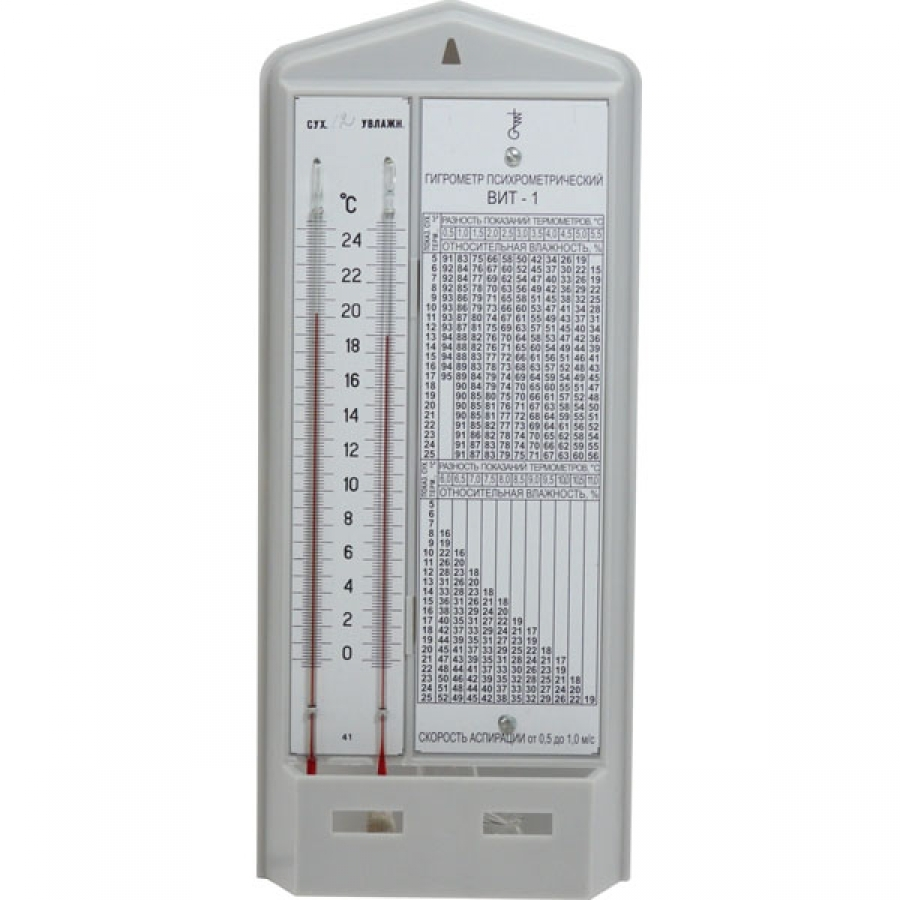
\includegraphics[width=0.5\textwidth]{./images/vit.jpg}
\caption{Гігрометричний психрометр ``ВИТ-1''}
\label{fig:vit}
\end{figure}

Прилад зображено на \ref{fig:vit}.

Метрологічні характеристики:
\begin{itemize}
\item Діапазон вимірювання відносної вологості --- $20 \ldots 90$ \%.
\item Температурний діапазон вимірювання вологості,  $5 \ldots 25$ °C.
\item Діапазон вимірювання температури $0 \ldots 25$°C.
\item Ціна поділки шкали термометрів:  $0.2$°C.
\end{itemize}

\subsection{Ємнісний електронний гігрометр ``Testo 605 H1''}
\begin{figure}[!ht]
\centering
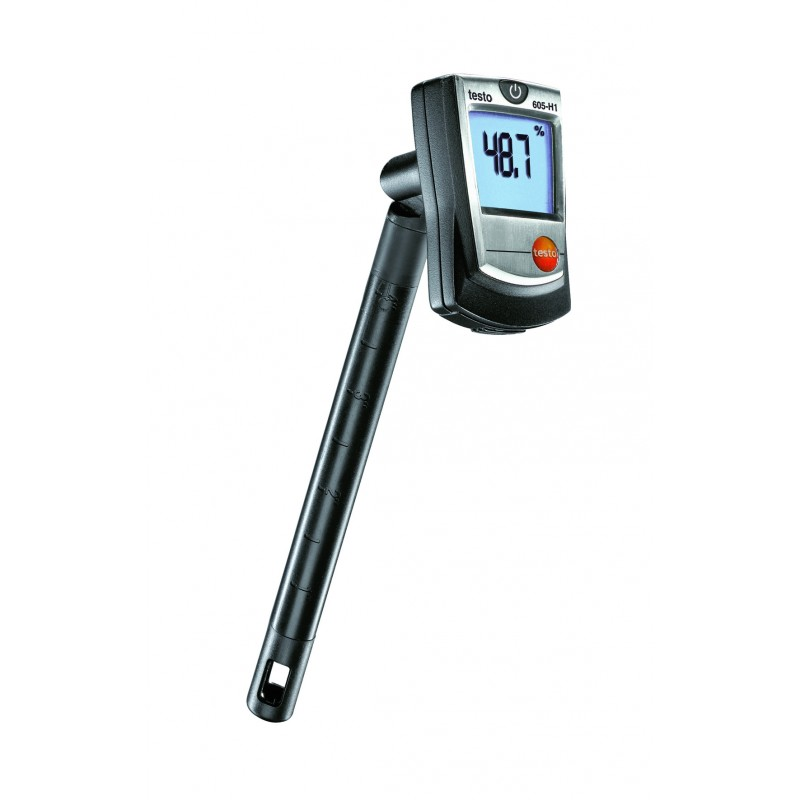
\includegraphics[width=0.5\textwidth]{./images/testo.jpg}
\caption{Ємнісний електронний гігрометр ``Testo 605 H1''}
\label{fig:testo}
\end{figure}

Прилад зображено на \ref{fig:testo}.

Метрологічні характеристики:
\begin{itemize}
\item Діапазон вимірювань --- $5 \ldots 95 \%$ ВВ;  $-10 \ldots +50$°C
\item Похибка --- $\pm 1\%$ ВВ
\item Робоча температура ---  $0 \ldots +50$ °С
\end{itemize}


\section*{Висновки до розділу 1}
\addcontentsline{toc}{section}{Висновки до розділу 1}

В цьому розіділі було розглянуто методи та засоби для вимірювання відносної волгоситі повітря.
На практиці застосовуються як прямі так і не прямі методи вимірювання.

Прямий метод: вимірювання вологості.

Непрямі методи: вимірювання ємності, опору та сили натягу.